% Basics
\part{Utilisation basique de git : Côté client}

\input{Setup}

\chapter{Commandes de base}

Nous allons enfin nous plonger dans le vif du sujet en voyant les commandes de bases de git et son fonctionnement.

\section{Créer un dépôt}

Contrairement à \acl{svn}, Git fonctionne à la fois en local et sur le serveur : chaque client contient son propre dépôt local.\\
Le dépôt en ligne ne permet que de synchroniser les différents dépôts locaux.\\

Pour commencer, nous allons travailler \textbf{hors-ligne} :

\subsection*{Par ligne de commande}
\begin{verbatim}
# Creer un dossier "test" et s'y rend
$ mkdir ~/test
$ cd ~/test

# Crée un dépôt dans le dossier courant
$ git init
\end{verbatim}

Voilà. C'est tout. Un dossier ".git" doit être apparu.
Sous git bash (sous windows) vous devriez voir une invite de commande indiquant la branche sur laquelle vous êtes (master).

Pour savoir si votre dépôt est actif, tapez :
\begin{verbatim}
$ git status

# En cas d'erreur :
fatal: Not a git repository (or any of the parent directories): .git

# En cas de réussite :
# On branch master
nothing to commit, working directory clean
\end{verbatim}

\subsection*{Par tortoise git}
Creez un nouveau dossier $\rightarrow$ Clic droit dessus $\rightarrow$ Create git repository here

Voilà. C'est tout. Un dossier ".git" doit être apparu.

Pour savoir si votre dépôt est actif, faites un clic droit : les options de tortoise git ont du changer.
Vous devirez pouvoir faire des commit, push, fetch, etc..

\begin{figure}[h] 
	\begin{center}
		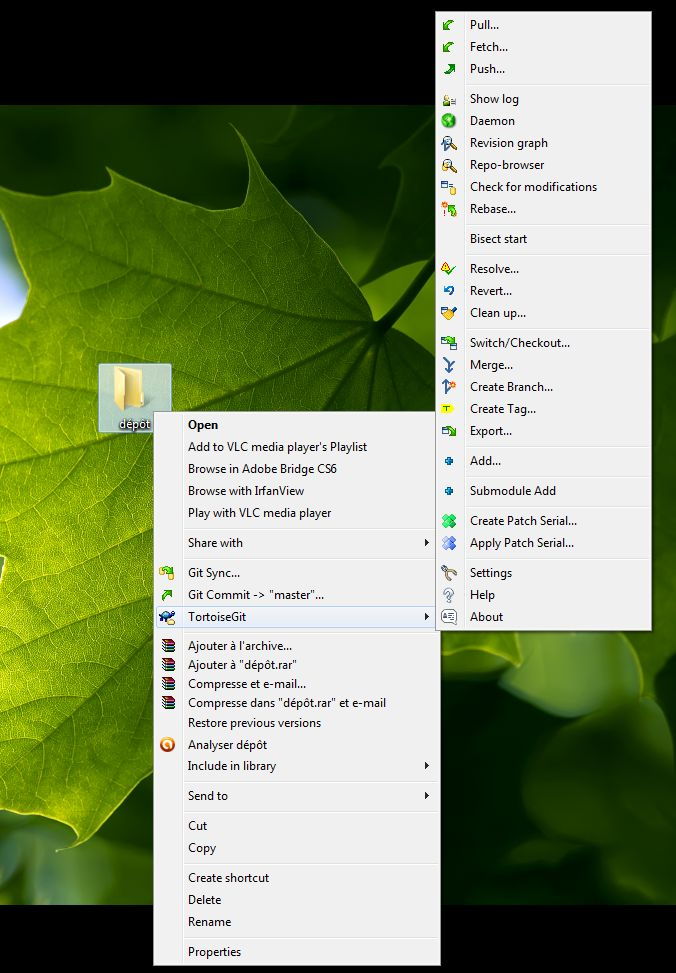
\includegraphics[scale=0.2]{../IMG/menuTG.jpg}
	\end{center}
	\caption{Tortoise Git : Le menu du depot}
	\label{Tortoise Git : Le menu du depot} 
\end{figure}
\newpage
\section{Un système de commits}

Git fonctionne un peu comme svn : par un système de version, ici appelés commit.\\
Pour commencer : créez un fichier nommé yoyo.txt et écrivez "Version 1" dedans.

A ce moment précis, vous considérez avoir bien travaillé et souhaitez \textbf{sauvegarder} votre travail dans git, de manière à le retrouver si jamais, plus tard, le fichier aurait un problème.

Nous allons donc créer une nouvelle version du projet.

\subsection{Indexer les fichiers}
Avant de créer un commit, nous devons dire à git quels fichiers doivent être pris en compte :
on appelle ça indexer les fichiers.
Indexer un fichier le mettra directement en cache, dans le dépôt.

\textbf{Attention : } Seuls les fichiers normaux et leur chemin sont mis en cache. Git en prend pas en compte les dossiers.\\
Si git veut nous créer un fichier sur notre ordinateur, si le dossier n'existe pas, il le fabrique.\\
Si on veut indexer un dossier vide, rien ne se passera.

\subsubsection{Par ligne de commande}
\begin{verbatim}
# Indexer le fichier1, le fichier2, et tous les fichiers du dossier3 (récursif)
$ git add <fichier1> [fichier2] [dossier3]

# Par exemple : indexe tous les fichier du dossier courant (et les ajoute au cache)
$ git add .

# Pour savoir quels sont les fichiers ajoutés, à ajouter, 
# modifiés (comparé au commit précédent)
$ git status
\end{verbatim}

Pour désindexer un fichier (supprimer le fichier et arrêter sa sauvegarde par le système de fichier), vous devrez passer par la commande git rm ou bien en supprimant au préalable le fichier et en utilisant l'option -A avec la commande git add.\\

Si vous souhaitez conserver le fichier dans votre système mais le retirer de l'index de git, il faut utiliser la commande git rm --cached

\subsubsection{Avec tortoise git}
Clic droit $\rightarrow$ Tortoise Git $\rightarrow$ Add

Tortoise git aide à l'indexation pendant le commit, il vous est en soi inutile de faire Add.\\
\newpage
\subsection{Créer un commit}
\subsubsection{Par ligne de commande}
\begin{verbatim}
# Créer un commit
$ git commit
\end{verbatim}

\textbf{Attention : } Vous allez entrer en mode texte (programme Vi) pour insérer un message.
Ici les lignes commançant par \# seront ignorées.
Pour éditer le texte, appuyez sur "i", pour arrêter l'édition, appuyez sur "Echap", pour valider le message :
arrêtez l'édition puis tapez ":wq"\\

Pour éviter de rentrer dans ce mode texte, vous pouvez écrire le message dans la commande :
\begin{verbatim}
# Créer un commit et tapez directement son message
$ git commit -m "Message"
\end{verbatim}

Pour indexer tous les fichiers qui ont été mis en cache :
\begin{verbatim}
# Créer un commit en indexant tous les fichiers mis en cache
$ git commit -a
\end{verbatim}

Vous pouvez aussi bien mélanger les options :
\begin{verbatim}
# Créer un commit en indexant tous les fichiers mis en cache
# et tapez directement son message
$ git commit -a -m "Message"
\end{verbatim}

\subsubsection{Par tortoise git}

Clic droit $\rightarrow$ Git Commit $\rightarrow$ "master"\\

Une fenêtre doit s'ouvrir contenant :
\begin{itemize}
\item Les fichiers mis en cache (avec une case cochée)
\item Les fichier non indexés (avec une case décochée)\\
\end{itemize}

La case indique s'il faut indexer ou non le fichier pour le commit à venir.
Si le fichier n'était pas en cache, il sera ajouté au dépôt et mis en cache\\

Une fois les fichiers choisis : tapez le message du commit (tentez d'être clair), signez, puis validez.\\

Vous pouvez aussi le faire directement depuis le log en faisant:
Clic droit $\rightarrow$ Tortoise git $\rightarrow$ Show log\\

Vous y verrez vos commits et les modifications courantes.\\
Pour créer un commit à partir de là : Clic droit sur "Working dir changes" $\rightarrow$ Commit
\newpage
\paragraph{Fenêtre de commit } Ici, le fichier toto.txt à été modifié, et le fichier nouveau.txt à été crée sans avoir encore été mis en cache/indexé.

\begin{figure}[h] 
	\begin{center}
		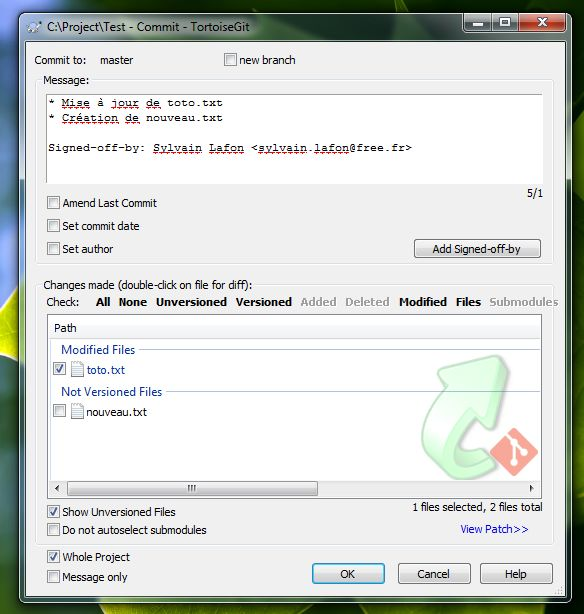
\includegraphics[scale=0.3]{../IMG/commit.jpg}
	\end{center}
	\caption{Tortoise Git : fenetre de commit}
	\label{Tortoise Git : fenetre de commit} 
\end{figure}

Pour ajouter le fichier nouveau, il suffit de cliquer sur la case à sa gauche.\\

\paragraph{Le log } Voici ce dont à quoi ressemble la fenêtre de log :

\begin{figure}[h] 
	\begin{center}
		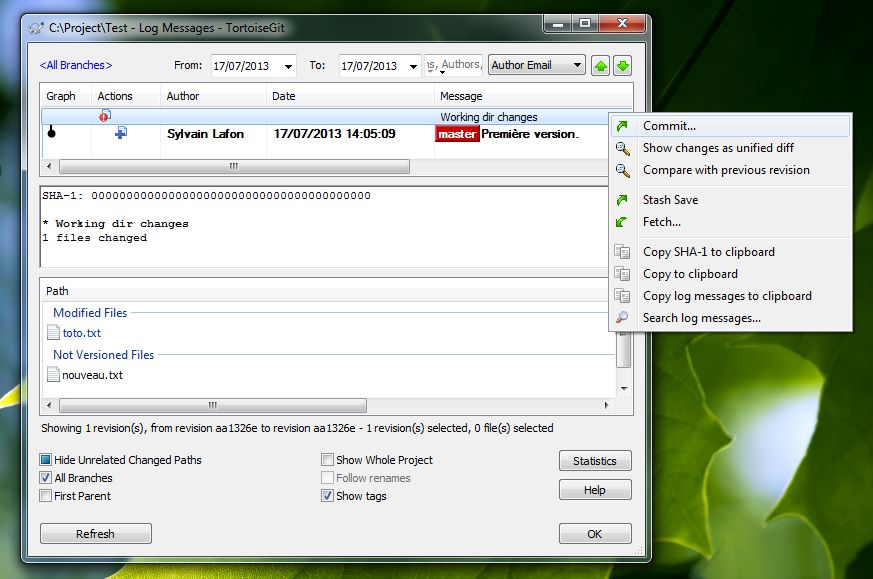
\includegraphics[scale=0.3]{../IMG/log.jpg}
	\end{center}
	\caption{Tortoise Git : fenetre de log}
	\label{Tortoise Git : fenetre de log} 
\end{figure}

Cette fenêtre doit être la fenêtre la plus importante de Tortoise git : elle permet d'afficher les commits en faisant leur graphe à leur gauche, en permettant, au clic droit de faire toutes les opérations que l'on verra.\\
Ici, un clic droit sur "Working dir. changes" permet de créer un commit,
on peut aussi faire des clics droit sur les branches, tags et commits.
\newpage
\subsection{Bien nommer les commits}

Idéalement, un commit devrait se présenter sous la forme suivante :
La première ligne devrait comporter moins de 50 caractères et résume les changements du commit.
Elle devrait être suivie d'une ligne blanche, puis des lignes qui décrivent plus en détail les différentes modifications.\\

Le texte situé au dessus de la ligne blanche est pris comme étant le titre du commit, utilisé dans git. (et Tortoise Git).\\
La commande git format-patch permet par exemple d'envoyer un commit par email et utilise le titre pour le sujet et le reste dans le corps du message.

\subsection{Se déplacer dans les commits}

Pour la suite du tutoriel,
faites deux nouveaux commits en modifiant le contenu de toto.txt

\subsubsection{Par ligne de commande}
\begin{verbatim}
$ git checkout <id>
\end{verbatim}

$<$id$>$ peut être un nom de branche, de tag ou bien l'id (SHA-1) du commit.
Pour connaitre les différents id de commit : 

\begin{verbatim}
$ git log --oneline --color --graph
\end{verbatim}

\subsubsection{Par tortoise git}
Clic droit $\rightarrow$ Tortoise git $\rightarrow$ Switch/Checkout
Une fenêtre apparait pour savoir vers où se déplacer, cochez "Commit" et ouvrez le log, cliquez sur la deuxième version puis "Ok", et "Ok".\\

Votre fichier a dû retrouver le contenu qu'il avait au deuxieme commit.\\

Vous pouvez aussi le faire directement depuis le log en faisant:
Clic droit $\rightarrow$ Tortoise git $\rightarrow$ Show log\\

Puis clic droit sur une version et "Switch/Checkout to this"
La version sur laquelle on se situe sera écrite en gras.
\newpage
\subsection{Référencer les commits importants : les tags}
Vous trouvez que certains commits sont très importants et vous y aimerez y accèder facilement, sans avoir à taper leur SHA-1 ? \\

Pour cela on utilise un tag. Il s'agit d'une simple référence à un commit, un nom.\\

Sur GitHub, une partie "Téléchargement" permet de télécharger le .zip du projet pour chaque tag !

\begin{figure}[h] 
	\begin{center}
		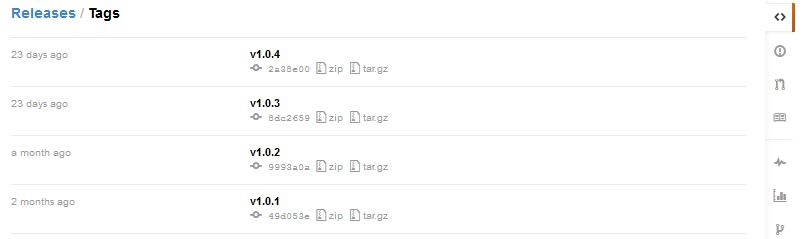
\includegraphics[scale=0.4]{../IMG/tagsdl.jpg}
	\end{center}
	\caption{GitHub : les tags}
	\label{GitHub : les tags} 
\end{figure}

\subsubsection{Par ligne de commande}
Pour commencer, allez sur le commit en question, puis utilisez "git tag"
\begin{verbatim}
# On va sur le commit dont le SHA-1 débute par abcdef
$ git checkout abcdef

# On y crée un tag nommé : "v1.0"
$ git tag v1.0

# On peut désormais y accèder en tapant "v1.0"
$ git checkout v1.0

# Pour SUPPRIMER un tag :
$ git tag -d v1.0
\end{verbatim}

\subsubsection{Par Tortoise Git}
Et par le log et par le menu, on a "Create tag".\\

Pour supprimer un tag, on doit forcément aller dans le log de tortoise git, puis faire un clic-droit sur le tag (en jaune) avant de cliquer sur Supprimer.
\newpage
\section{Un système de branches}

Puisque nous pouvons travailler en parallèle où bien vouloir modifier un fichier à partir d'une version plus récente :
git utilise ce que l'on appelle des branches.\\

\subsection{Commits, branches et HEAD}

Par défaut, nous avons 3 choses :
\begin{verbatim}
A     B     C
* --- * --- *
        HEAD=master
\end{verbatim}

\begin{description}
\item[- Les commits : ] sont représentés par les * : A, B et C.\\
Ils ont chacun un identifiant SHA-1.\\
\item[- Les branches : ] ici, il n'y a que master.\\
Une branche fait parti de ce que l'on appelle une référence, dans git. Elles sont représentées par un fichier qui se situe dans .git/refs/heads et qui contient le SHA-1 du commit où elles se trouvent.\\
\item[- HEAD : ] Il s'agit de l'endroit sur lequel on est.\\
Unique, HEAD fait aussi parti de ce que l'on appelle une référence, mais celle-ci est particulière étant donné qu'elle peut à la fois pointer sur un commit, mais aussi sur une autre référence (ex: une branche).\\
Il est représenté par le fichier /.git/HEAD.\\
\end{description}

\textbf{Attention : }Si HEAD se trouve sur le même commit qu'une branche, cela ne veut pas dire que HEAD pointe forcément sur une branche !\\

Dans mes schémas, si HEAD ne pointe pas sur un commit mais sur une branche, j'utiliserai le symbole =. Dans le schéma ci-dessus : HEAD pointe sur master.
\newpage
Sur Tortoise Git, HEAD est représenté par le gras.
Si HEAD se trouve sur une branche, le nom de la branche en question est mis en rouge.\\

Lorsque l'on crée un commit, il est crée à partir du commit où se trouve HEAD, et il peut se passer deux choses :\\
\begin{itemize}
\item si HEAD pointe sur un commit : HEAD pointe sur le nouveau commit
\item si HEAD pointe sur une branche : la branche pointe sur le nouveau commit, HEAD pointe toujours sur la branche (la branche grandit)\\
\end{itemize}

\begin{verbatim}
A     B     C                A     B     C     D
* --- * --- *       ====>    * --- * --- *
    HEAD  master                   |   master
                                   ----------- *
                                              HEAD
          
A     B     C                A     B     C     D
* --- * --- *       ====>    * --- * --- * --- *
           HEAD                        master HEAD
          master                          
          
          
A     B     C                A     B     C     D
* --- * --- *       ====>    * --- * --- * --- *
        HEAD=master                        HEAD=master
        
\end{verbatim}

Dans le cas où l'on sort d'une branche non référencée, nous risquons de perdre tout les commits qu'elle apportait.
Pour éviter que cela n'arrive, nous allons commencer par apprendre à créer une nouvelle branche.

\begin{verbatim}
A     B     C     D            A     B     C     D
* --- * --- *                  * --- * --- *
      |   master       ====>         | HEAD=master
      ----------- *                  ----------- *
                 HEAD                         (perdu)
\end{verbatim}
\newpage
\subsection{Créer une branche}
\subsubsection{Par ligne de commande}

Par défaut, la branche que vous créerez se situera à l'endroit où se trouve HEAD.
Il y a deux méthodes pour créer une branche :

\begin{verbatim}
# Créer une branche et y faire pointer HEAD
$ git checkout -b <nom_branche>

# Créer une branche sans y faire pointer HEAD
$ git branch <nom_branche>
\end{verbatim}

\subsubsection{Par Tortoise Git}
\begin{itemize}
\item Clic droit $\rightarrow$ Tortoise Git $\rightarrow$ Create branch
\item Log $\rightarrow$ Clic droit sur une version $\rightarrow$ Create branch at this version
\item Lors d'un commit : case "New branch", la branche sera crée et HEAD pointera dessus avant que le commit ne se crée
\end{itemize}

\subsubsection{Résultat}
\begin{verbatim}
A     B     C                A     B     C     D
* --- * --- *       ====>    * --- * --- *
    HEAD  master                   |   master
                                   ----------- *
                                              HEAD                                              

                    ====>    A     B     C     D
                             * --- * --- *
                                   |   master
                                   ----------- *
                                         HEAD=maBranche
\end{verbatim}

\newpage
\subsection{Déplacer HEAD}

Il y a plusieurs méthodes pour faire déplacer HEAD :\\

\begin{verbatim}
# Déplace HEAD proprement, mélange les modifications en cours avec  
# celles induites par le déplacement dans les versions.
# Empêche le déplacement en cas de conflits dans le mélange des modifications.
$ git checkout <ref>

# Déplace HEAD en SUPPRIMANT toutes les modifications en cours.
$ git reset --hard <ref>

# Déplace HEAD mais conserve les fichiers du précédent commit et les indexe
# Les modifications en cours seront la différence entre le commit cible 
# et le commit précédent en plus des modifications qu'il y avait
$ git reset --mixed <ref>

# Déplace HEAD mais conserve les fichiers du précédent commit et ne les indexe pas
# Cela revient à modifier /.git/HEAD
$ git reset --soft <ref>
\end{verbatim}

Il est possible de faire l'ensemble de ces opérations avec tortoise git à partir du log : Faites un clic droit sur la branche ou le commit qui vous intéresse et choisissez Checkout ou Reset. Si vous choisissez reset, vous aurez le choix entre les trois modes.

\newpage

\subsection{Fusionner la branche courante}

Bien évidemment, si on ne pouvait pas stocker les changements quelle apporte dans la branche principale, la création d'une nouvelle branche ne servirait à rien.
Nous allons donc apprendre à mettre à jour une branche en la fusionnant avec HEAD.

Pour pouvoir fusionner deux branches il faut, pour commencer, que la branche à fusionner apporte des changements à la branche courante.\\

Par exemple :
\begin{verbatim}
A       B       C
* ----- * ----- *
      aMerger 
            HEAD=master
\end{verbatim}

Il est absolument inutile dans ce cas de fusionner aMerger dans master !
master contient déjà toutes les modifications de aMerger.
\newpage
\begin{verbatim}
A       B       C               A       B       C
* ----- * ----- *               * ----- * ----- *
   HEAD=master          ====>               HEAD=master
              aMerger                         aMerger
\end{verbatim}

Là, par contre, bien que master n'apporterait rien à aMerger, ici,
aMerger contient des modifications que master n'a pas. Fusionner master et aMerger permettrait de mettre à jour master.

\begin{verbatim}
A     B     C     D             A        B        C        D         M
* --- * --- *     *             * ------ * ------ * ---------------- *      
      | HEAD=master     ====>            |                           |
      ----------- *                      ----------------- * ---------
                aMerger                                 aMerger  HEAD=master
                                                      (fusionnée)
\end{verbatim}

Ici, les deux branches ont eu des changements parallèles : une véritable fusion entre les fichiers à lieu, ce qui crée un commit de fusion.
Git est assez puissant et arrive facilement à faire la part des choses, cependant parfois les mêmes endroits des mêmes fichiers sont modifiés, on appelle ça un conflit : il faut, dans ce cas, le résoudre à la main. On en parlera plus tard. \\

Donc maintenant, comment fusionner les branches ?
\subsubsection{En lignes de commande}
\begin{verbatim}
# Faites attention que vous n'ayez rien à commiter !
$ git status

# D'abord on se place sur la branche que l'on veut
$ git checkout aMettreAJour

# Puis on fusionne !
$ git merge aMerger

# Résultat
$ git log --oneline --color --graph
\end{verbatim}

\subsubsection{Par Tortoise git}
Vous devriez être déjà plus familier avec l'interface.
Le bouton à appuyer s'appelle "Merge".
Il faut tout d'abord veiller à bien être sur la branche qui recevra la fusion.
On peut trouver le bouton et dans le log et dans le menu clic-droit.
\newpage
\subsection{Résoudre les conflits}

Arg, votre fusion ne s'est pas faite toute seule et git vous supplie de l'aider ?
Pas de soucis, on va les résoudre ces conflits !!

Lorsque git ne sait pas quoi faire, il va écrire localement tous les confits dans le fichier

Par exemple :
Ecrivons dans notre fichier toto :
\begin{verbatim}
A
B
C
D
E
\end{verbatim}

Créons un commit, et retournons au commit précédent\\

\textbf{Astuce} Pour la ligne de commande : HEAD$^{\bigwedge}$1 indique : "un commit avant HEAD"\\

Créons une nouvelle branche "troll" écrivons dans le fichier toto :
\begin{verbatim}
A
bbbbb
C
ddddd
E
\end{verbatim}

Créons un commit, nous devrions avoir un graph qui ressemble à ça :

\begin{verbatim}
                     A      B      C
anciens commits ---- * ---- *
                     |    master
                     ------------- *
                               HEAD=troll
\end{verbatim}

Maintenant, retournons (HEAD) sur master et fusionnons troll à HEAD(=master).

La fusion se place pas comme prévue (enfin..) et git vous indique qu'il a besoin d'aide.
A ce moment précis, toutes les modifications apportées par troll sont indexées, et les fichiers non fusionnés sont notés comme "conflictueux"
\newpage
Git, pour vous aider, à écrit dans toto de cette manière :
\begin{verbatim}
A
<<<<<<< HEAD
B
C                                <-- Partie telle qu'elle est dans HEAD
D
=======
bbbbb
C                                <-- Partie telle qu'elle est dans troll
ddddd
>>>>>>> troll
E
\end{verbatim}

Pour résoudre le conflit vous devez alors supprimer les annotations supplémentaires et fusionner la partie problématique.
Pour indiquer à git que le conflit est résolu il suffit d'indexer le fichier (git add) ou de le supprimer (git rm) et pour finir la fusion, il faut créer le commit de fusion (il est impossible de faire de commit s'il reste des fichiers conflictueux)

\subsubsection{En ligne de commande}

Vous pouvez faire revenir un fichier selon l'une ou l'autre branche à l'aide de checkout :
\begin{verbatim}
# Marque toto.txt comme résolu :
$ git add toto.txt

# Résout le conflit en prenant le fichier de HEAD(=master)
$ git checkout --ours toto.txt

# Résout le conflit en prenant le fichier de la branche à fusionner (troll)
$ git checkout --theirs toto.txt
\end{verbatim}

\subsubsection{Sous tortoise git}

Tout comme en ligne de commande, sous Tortoise Git, il y a des outils facilitant la résolution des conflits. Des outils de feignants certes, mais bien utiles.\\
Après la tentative de fusion, git vous propose de "Résoudre" les conflits, si vous acceptez : la fenêtre de commit normale apparait (sinon il suffit de cliquer sur "Commit")\\

Ici, Tortoise git propose trois choses (clic droit sur les fichier à conflit) :
\begin{itemize}
\item Résoudre le conflit (il faut faire les modifications à la main avant)
\item Résoudre le conflit en prenant la version locale (celle de HEAD)
\item Résoudre le conflit en prenant la version distante (celle de troll)\\
\end{itemize}

Bien sûr il reste aussi possible de le supprimer.
\newpage
\subsection{Supprimer une branche}

Pour commencer : on ne peut pas supprimer une branche si HEAD est dessus, ensuite, pour supprimer une branche \textbf{sans forcer}, elle doit être fusionnée, par exemple :
\begin{verbatim}
__________________________________________________

 A        B        C        D         M
 * ------ * ------ * ---------------- *      
          |                           |            
          ----------------- * ---------
                         aMerger  HEAD=master
                       (fusionnée)
                       
> Aucun risque de supprimer aMerger
__________________________________________________
                       
 A        B        C        D        
 * ------ * ------ *      
          |    HEAD=master                         
          |                                        
          ----------------- *                      
                         branche1 (fusionnée à branche2)
                         branche2 (fusionnée à branche1)

> Aucun risque de supprimer branche1 ou branche2
__________________________________________________

 A        B        C        D        
 * ------ * ------ *      
          |    HEAD=master                         
          |                                        
          ----------------- *                      
                         branche1

> Supprimer branche1 risque de perdre D .       
\end{verbatim}
(Un commit perdu n'est pas tout de suite supprimé : il restera accessible avec son SHA-1 quelques temps. (cf : git prune))\\

Si la branche n'est pas fusionnée, il va falloir forcer, à ce moment là, on peut supprimer la branche "aMerger" sans aucun problème, et sans perdre quoi que ce soit.
\newpage
\subsubsection{En ligne de commande}
\begin{verbatim}
# On s'assure de ne pas être sur aMerger
$ git checkout master

# On la supprime (si fusionnée)
$ git branch -d aMerger

# On la supprime (en forcant)
$ git branch -D aMerger
\end{verbatim}

Par sécurité, il est conseillé de ne jamais forcer (sauf si vous vous fichez de perdre le travail qui n'a pas été fusionné).

\subsubsection{Avec tortoise git}
Sur la version de Tortoise git que j'ai actuellement : on est obligé d'ouvrir le log pour supprimer une branche (clique-droit sur une branche (en vert))\\

\textbf{Attention} : Cela forcera la suppression automatiquement, alors soyez vigilants !

\newpage
\section{Un dépôt en ligne}
L'un des grands avantages d'utiliser git, en plus de pouvoir gérer facilement les versions hors-ligne (ce qui le démarque de \acl{svn}), c'est aussi la possibilité de synchroniser ses branches sur un serveur en ligne rendant ainsi possible la mise en commun des différentes versions\\

Lorsque l'on lie notre dépôt à un dépôt distant, on peut :
\begin{description}
\item[- fetch :]Recevoir les branches en ligne (et les commits de différence)
\item[- push :] Créer/Fusionner (commit de fusion interdit) une de nos branches, dans le serveur
\end{description}

Commençons par lier notre dépôt à un dépôt en ligne.

\subsection{Lier un dépôt local à un dépôt serveur}
\subsubsection{Par ligne de commande}
\begin{verbatim}
$ git remote add <nom identifiant du dépôt> <adresse du dépôt>

# Par défaut on appelle le premier identifiant "origin"

# Exemple pour github, par ssh :
$ git remote add origin git@github.com:nomUtilisateur/nomDepot.git

# Exemple pour github, par https :
$ git remote add origin https://github.com/nomUtilisateur/nomDepot.git
\end{verbatim}

\subsubsection{Par Tortoise git}
Clic droit $\rightarrow$ Tortoise git $\rightarrow$ Settings $\rightarrow$ Git $\rightarrow$ Remote\\

Ici, on renseigne les champs "Remote" et "URL", avant d'appuyer "Add New/Save" puis "Ok"\\

Par exemple : "origin" et "git@github.com:nomUtilisateur/nomDepot.git" pour github

\newpage
\subsection{Créer un clone d'un dépôt en ligne}

Créer un clone d'un dépôt permet d'obtenir un dépôt local identique au dépôt en ligne, directement lié avec le dépôt en ligne. (l'identifiant sera "origin").

\subsubsection{Par ligne de commande}
\begin{verbatim}
$ git clone <adresse du dépot> [nom du dossier (optionnel)]

# Exemple pour github, par ssh :
$ git clone git@github.com:nomUtilisateur/nomDepot.git

# un dossier "nomDepot" sera crée

# Exemple pour github, par ssh :
$ git clone git@github.com:nomUtilisateur/nomDepot.git nomDossier

# un dossier "nomDossier" sera crée
\end{verbatim}

\subsubsection{Tortoise git}
Clic droit en dehors d'un quelconque dépôt, puis Clone.
On remplit l'url, et c'est parti !

\subsection{Récupèrer les différences avec le serveur}
Pour récupèrer les modifications qui se sont faites en ligne, il suffit de faire un "fetch"
(git fetch).

Si des commits existent en ligne mais pas en local, ils seront téléchargés.

Exemple :
\begin{verbatim}

          A     B     C
local :   * --- * --- *     
                  HEAD=master

ORIGIN    A     B     C     D
remote :  * --- * --- * --- *
                        HEAD=master
   
<<FETCH ORIGIN>>

          A        B        C        D         
local :   * ------ * ------ * ------ *
                        HEAD=master
                          origin/HEAD=origin/master
\end{verbatim}

Pour mettre à jour master, il suffit de faire un merge de origin/master !\\

Faire les deux opérations à la suite, c'est faire faire un pull (git pull)

\subsection{Fusionner une branche distante}
Pour mettre à jour le serveur, faire un Push, il faut au préalable que notre branche soit déjà fusionnée avec la branche à fusionner.. concrètement :
\begin{verbatim}
A     B     C
* --- * --- *             <-- Déjà à jour.
          master
       origin/master

A     B     C
* --- * --- *             <-- Possible
          master   
  origin/master
  
A     B     C
* --- * --- *             <-- Pas possible (inutile)
          origin/master   
    master
           
A     B     C     D
* --- * --- *             <-- Pas Possible (non fusionnée : conflit possible)
      |   master  
      ----------- *     
            origin/master
\end{verbatim}

\subsection{Astuce : Le protocole habituel}
Habituellement, lorsque l'on veut envoyer notre version en ligne, on fait, ces opérations dans l'ordre :

\begin{enumerate}
\item ADD : On indexe les modifications et on met en cache les nouveaux fichiers
\item COMMIT : On crée un commit, une version
\item FETCH : On récupère la version en ligne
\item MERGE : On fusionne la version en ligne avec la version locale
\item PUSH : On envoie la nouvelle version locale en ligne\\
\end{enumerate}

Puisque un commit peut faire un "add" et que le fetch et merge se font avec la commande "pull", on peut résumer le protocole à :\\

\begin{enumerate}
\item COMMIT EN INDEXANT (commit -a / les cases de tortoise)
\item PULL (FETCH + MERGE)
\item PUSH
\end{enumerate}
\newpage
\subsection*{Lignes de commande}
\begin{verbatim}
# récupèrer pour toutes les remotes
$ git fetch 

# récupèrer que pour origin
$ git fetch origin

# récupèrer pour toutes les remotes et merger toutes les branches
$ git pull

# récupèrer que pour origin et merger toutes les branches
$ git pull origin

# récupèrer que pour origin et ne merger que master
$ git pull origin master

# tout envoyer sur toutes les remotes
$ git push

# tout envoyer sur origin
$ git push origin

# envoyer master sur origin
$ git push origin master

# envoyer master en tant que "maBranche" sur origin
$ git push origin master:maBranche
\end{verbatim}

\subsection{Supprimer une branche distante}
\subsubsection{Par ligne de commande}
On va utiliser l'option --delete de push :
\begin{verbatim}
# détruit et la branche locale origin/maBranche et la branche maBranche d'origin
$ git push origin --delete maBranche
\end{verbatim}
\subsubsection{Par tortoise git}
Dans le log, clic droit sur une remote/branche et supprimer : une popup apparaîtra pour savoir s'il faut ou non supprimer ET la branche locale (remote/branche) ET la branche "branche" sur le dépôt en ligne.

% Fait sauter une page dans le Table of contents
\addtocontents{toc}{\protect\newpage}